\section{Introduzione}
\label{section:introduzione}

Il capitolo corrente fa da introduzione al lavoro svolto e orienta il lettore 
ad alcuni aspetti principali relativi al campo dello ``Spreading Rumors''.

I primi studi riguardanti la diffusione di una notizia risalgono ai primi anni '60~\cite{biblio:stochastic_rumours}, 
ma quelli presi in considerazione in questo lavoro sono più attuali e riguardano il campo dei Social Networks.

Lo studio della propagazione di una ``voce'', definita più semplicemente notizia o informazione, 
serve ad analizzare alcuni comportamenti, paramenti e modelli di una rete sociale.
Le caratteristiche principali studiate sono la topologia della rete e gli utenti che ne fanno parte.

Possiamo quindi dire che le simulazioni prevederanno una rete di utenti che, ``a contatto'' con
la notizia, decideranno se ricondividerla o se solamente prenderne atto.
Al passo 0 della simulazione verrà scelto un utente a cui verrà ``insegnata'' l'informazione da propagare. 
Facendo un riferimento al tema della medicina, durante un'indagine epidemiologica, il primo paziente ad aver 
contratto la malattia viene chiamato paziente zero; nella situazione in questione, anzichè di una malattia, si tratterà di una notizia

Durante le simulazioni verranno inoltre utilizzati alcuni termini che definirò di seguito:
\begin{itemize}
 \item ``Ignorants''\cite{biblio:spread_rumor} : al momento della creazione della rete sociale tutti gli utenti vengono definiti 
 in tal modo, in quanto non al corrente della notizia;
 \item ``Spreaders''\cite{biblio:spread_rumor} : tutti gli utenti che decidono di condividere la notizia. 
 Il ``paziente zero'' viene incluso in questo gruppo;
 \item ``Uninterested'' : tutti quegli utenti che dopo aver appreso la notizia, decidono di non condividerla;
 \item ``Viewers'' o visualizzatori : tutti coloro facenti parte del gruppo degli Spreaders e degli Uninterested.
\end{itemize}

Facendo una veloce panoramica, l'argomento di questo progetto è certamente un ottimo ambiente di studio; 
inoltre il numero esorbitante di utilizzatori di Social Networks in circolazione crea, sicuramente, 
un terreno fertile per la diffusione di notizie ed informazioni.



\subsection{Obiettivi}
\label{section:obiettivi}

Per questo lavoro si possono inquadrare tre obiettivi principali.

Il primo test permetterà di decidere il modello topologico più consono, tra quelli 
presi in considerazione, per i successivi test.

Il secondo test servirà per mettere in luce come una notizia, 
con un topic adatto maggiormente ad una certa fascia d'età, venga diffusa nei differenti Social Networks.
On-line è presente una statistica piuttosto recente (3\degree trimestre 2014) che mostra una distribuzione 
relativa alla divisione, per età, dell’utenza nei social networks più popolari. 
Il grafico in figura~\ref{img:age_distribution_social} ne mostra la distribuzione.

\begin{figure}[!ht]
 \centerline{
  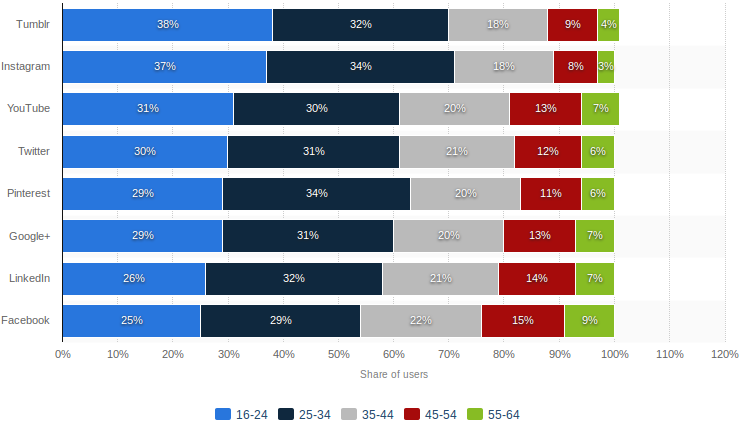
\includegraphics[width=0.8\textwidth]{img/age-distribution.png}
 }
\caption{Distribuzione delle età divisa per Social Network ~\cite{biblio:age_distribution_social}}
\label{img:age_distribution_social}
\end{figure}


Il terzo, ed ultimo, test ha come obiettivo, invece,  l'analisi di un’interazione tra 2 diversi gruppi di utenti e 
permetterà di studiare il numero di visualizzazioni della notizia in casi più complessi.
Un esempio potrebbe essere quello di dividere il numero totale delle persone in due sottoinsiemi così formati:
\begin{itemize}
 \item Il primo gruppo è formato da pochi utenti, ad esempio il 20\% del totale, ma ogni componente ha un'ottima probabilità di condivisione.
 \item Il secondo gruppo, viceversa, è formato dall'80\% degli utenti, ma ogni componente ha una possibilità minore di condivisione.
\end{itemize}





